\documentclass[12pt]{report}
\usepackage[utf8]{inputenc}
\usepackage{nameref}
\usepackage{fancyhdr}
\usepackage{hyperref}
\usepackage{caption}
\usepackage{csquotes}
\usepackage{indentfirst}
\usepackage[superscript,biblabel]{cite}
\usepackage{boldline}
\usepackage{graphicx}
\usepackage{float}
\usepackage{listings}
\renewcommand{\contentsname}{Sisukord}
\renewcommand{\bibname}{Kasutatud materjalid}
\renewcommand{\thesection}{\arabic{section}}
% Page numbers to the right
\pagestyle{fancy}
\fancyhead{}
\fancyfoot{}
\fancyfoot[R]{\thepage}
\renewcommand{\headrulewidth}{0pt}
% Code formatting
\newcommand{\code}[1]{\texttt{#1}}

\title{Versiooniuuenduse raamistik kasutades skriptimiskeelt Bash}
\author{Irina Ivanova}
\date{January 2016}

\begin{document}
  \begin{titlepage}
    \begin{center}
      TARTU ÜLIKOOL\\
      MATEMAATIKA-INFORMAATIKATEADUSKOND\\
      Arvutiteaduse instituut\\
      Infotehnoloogia eriala
    \end{center}
      
    \vspace{5cm}
    
    \begin{center}  
      {\Large Irina Ivanova}
    \end{center}
    \begin{center}      
      {\huge Versiooniuuenduse raamistik}
    \end{center}
    \begin{center}
      {\huge kasutades skriptimiskeelt Bash}
    \end{center}
    \begin{center}
      {\large Bakalaureusetöö (6 EAP)}
    \end{center}
      
    \vspace{4cm}
    \hspace{4.5cm}
    Juhendajad: dotsent Helle Hein
    
    \hspace{7cm}
    Polina Morozova, MSc (Nortal AS)
      
    \vspace{2.5cm}
    \begin{center}
      TARTU 2016
    \end{center}
  \end{titlepage}

  \newpage
  
  \noindent{\textbf{Versiooniuuenduse raamistik kasutades skriptimiskeelt Bash}}\\
  
  \noindent{\textbf{Lühikokkuvõte:}}\\
  \vspace{2cm}
  
  \noindent{\textbf{Võtmesõnad:}}\\
  Bash skript, versiooni uuendus, Apache Tomcat, Java
  \vspace{2cm}

  \noindent{\textbf{Thesis title}}\\

  \noindent{\textbf{Abstract:}}\\
  \vspace{2cm}

  \noindent{\textbf{Keywords:}}\\
  Bash script, version update, Apache Tomcat, Java
  
  \newpage
 
  \tableofcontents
  \fancypagestyle{plain}{%
    \renewcommand{\headrulewidth}{0pt}%
    \fancyhf{}%
    \fancyfoot[R]{\thepage}%
  }
 
  \newpage
  
  % Sissejuhatus
  \section*{Sissejuhatus}
  \label{sissejuhatus}
  \addcontentsline{toc}{section}{\nameref{sissejuhatus}}
  
  Käesolevas lõputöös lahendatakse rakenduslikku probleemi toimivas tarkvaraprojektis. Probleem seisneb selles, et projekti olemuse tõttu toote versiooni uuendamise protsess võtab kaua aega ja eeldab palju manuaalset sekkumist. See raiskab resursse ja suurendab inimliku vea tekkimise tõenäosust. Töö eesmärk on automatiseerida versiooniuuenduse protsessi konkreetses projektis, selleks, et lihtsustada antud protsessi, et säästa aega ja vähendada inimlike vigade arvu.\\
  
  Töö koosneb viiest osast. Esimeses osas püstitatakse probleem: kirjeldatakse projekti arhitektuuri, manuaalse uuendamise protsessi, probleeme, mis vana protsess toob ja nõudeid uuele lahendusele. Peamine väljakutse seisneb selles, et toode koosneb paarkümnest moodulitest (täpne arv sõltub kliendi nõuetest), mida on vaja paigaldada 31 keskkonna. See tähendab, et selleks, et paigaldada toote uut versiooni kõikidele keskkondadele on vaja teha umbes 620 uuendust (mitte arvestades testkeskkondade vaheuuendustega). Lisaks on projektis kasutusel kaks erinevat veebiserverit: Oracle WebLogic 12 ja Apache Tomcat 8. Uuenduse protsessi automatiseerimine peab võtma arvesse kõik need väljakutsed.\\
  
  Teises osas uuritakse võimalikke lahendusi: kas kasutada turul olemasolevat toodet (töös uuritakse neli toodet: Atlassian Bamboo, Chef, Jenkins ja Ansible Tower) või kirjutada ise tarkvara. Tuuakse välja iga lahenduse eeliseid ja puuduseid ning seletatakse miks langetati otsus Bash skripti kirjutamise kasuks. Valmistoodete peamised puudused on maksmus, võimetus hallata protsesse ja vajadusel parandada vigu, vajadus kulutada palju aega toode tundmiseks ja rakendamiseks.\\
  
  Kolmandas osas kirjeldatakse valitud lahendust: mis on skripti tööpõhi-mõtte ja arhitektuur ja kuidas seda saab paigaldada ja kasutada. Skripti põhifunktsionaalsus on mooduli faili alla laadimine, vana versiooni maha võtmine, uue versiooni paigaldamine, kolleegide teavitamine toimunud versiooniuuendusest. Lisaks oluliseks funktsionaalsuseks on erinevad kontrollid, mis vähendavad tõenäosust paigaldada vale versioon ja logimise funktsionaalsus, mis võimaldab kätte saada põhjalikku infot iga uuenduse kohta.\\
  
  Neljandas osas uuritakse kuidas antud lahendus mõjus projektile: võrrel-dakse versiooni uuendusele kulunud aega manuaalse ja automatiseeritud protsessi puhul ja lisatakse kolleegide tagasisidet uue raamistiku kasutamisele.\\
  
  Viimases osas tuuakse välja lahenduse perspektiive: kuidas loodud skripti saab edasi arendada ja kuidas saab seda teistes projektides rakendada.\\
  
  Töö tulemuseks on töötav, avatud lähtekoodiga, skript Bash keeles ja selle dokumentatsioon.
  
  \newpage
  
  % Probleem
  \section{Probleemi püstitus}
  
  Versioonide uuendamine on tingimata vajalik protsess tarkvara arenduses. Projektis, mida kirjeldatakse käesoleva töö raames, see protsess mängib väga olulist rolli.\\
  
  Projekti rakendus on kirjutatud Java keeles ja on kasutusel .WAR failid. Lisaks projekt rakendub modulaarsuse süsteemi, mis tähendab, et kogu rakenduse kood on jagatud moodulite kaupa ja iga mooduli kohta on olemas eraldi .WAR fail. Kokku on umbes 20 moodulit (täpne arv sõltub kliendist, sest erinevatel klientidel on erinev moodulite komplekt).\\
  
  Rakendust kasutavad 10 klienti. 3-l nendes on olemas 3 keskkonda: toode, demo (kus kliendid tutvuvad uue funktsionaalsuse ja parandustega enne toote uuendust) ja test (kus projekti meeskond testib funktsionaalsust enne tarnimist kliendile). 7-l kliendil on olemas 2 keskkonda: toode ja test. See tähendab, et kokku on olemas $3*3+7*2=23$ kliendikeskkonda. Lisaks veel umbes 7 projekti test keskkonda, mida kasutatakse erinevatel faasidel erineva funktsionaalsuse testimise jaoks. Seega kokku tuleb $23+7=30$ keskkonda, mida on vaja regulaarselt uuendada (mitte arvestades lokaalsete ja virtuaalmasinatega, mida iga meeskonnaliige võib vajadusel panna püsti). See tähendab, et selleks, et paigaldada rakenduse uut versiooni igale keskkonnale on vaja teha $30*20=600$ uuendust.\\
  
  Toodud numbrid näitavad, et versiooni manuaalne uuendus võtab palju aega ja tähelepanu, mille pärast oli otsustatud lihtsustada ja automatiseerida uuenduse protsessi.
  
  \newpage
  \subsubsection{Manuaalne uuenduse protsess}
  
  Ühe mooduli manuaalse uuenduse protsessi sammud on nimetatud allpool tabelis 1 "Manuaalse uuenduse protsessi sammud".
  
  \begin{table}[H] 
  \begin{tabular}{ |c|p{11cm}| }
    \hline
    \textbf{Number} & \textbf{Samm}\\
    \hline
    1 & .WAR faili uue koodiga alla laadimine serveri peale.\\
    \hline
    2 & Kui veebiserveriks on Oracle WebLogic, siis .WAR faili prekompileerimine (Apache Tomcat veebiserveril seda sammu ei ole).\\
    \hline
    3 & Faili ümber nimetamine.\\
    \hline
    4 & Faili paigaldus.\\
    \hline
    5 & Vana faili eemaldamine.\\
    \hline
    6 & Uue versiooni staatuse kontrollimine.\\
    \hline
    7 & JIRA töö uuendamine, mis automaatselt saadab emaile kolleegidele, et versioon on uuendatud (iga mooduli ja keskkonna kohta on olemas eraldi JIRA töö).\\
    \hline
    8 & Alla laaditud faili kustutamine.\\
    \hline
  \end{tabular}
  \caption*{\textit{Tabel 1: Manuaalse uuenduse protsessi sammud}}
  \end{table}
  
  Mitmete moodulite uuendamisel tuleb teha kõik need sammud iga mooduli jaoks. Aeg, mida võtavad need sammud, sõltub moodulist (kuna mõnes moodulis võib olla kaks korda rohkem koodi, kui teises, mis tähendab, et selle alla laadimine ja paigaldamine võtab kaks korda rohkem aega), aga keskmiselt see on 1.5 minutit. Kõikide moodulite uuendamine võib võtta tund aega, kuna lisandub veel aeg, mida inimene raisab õige versiooni numbri leidmiseks, .WAR faili aadressi kopeerimiseks, õige JIRA töö leidmiseks ja avamiseks jne. See tähendab, et inimlike vigade tekkimise tõenäosus on suur (nt alla laadida vale versiooni).\\
  
  Allpool on toodud Tabel 1 "Nõuded versiooni uuenduse lihtsustamise lahendusele", mis kirjeldab lahendust, millele on mõtet investeerida aega protsessi muutmiseks \--- muul juhul uue protsessi loomine võtab rohkem aega, kui toob kasu.
  
  \begin{table}
  \begin{tabular}{|c|p{11cm}|}
    \hline
    \textbf{Number} & \textbf{Nõue}\\
    \hline
    1 & Uuenduse protsess peab võtma vähem aega.\\
    \hline
    2 & Uuenduse protsess peab nõudma nii vähe käsitsi tegevusi, kui on võimalik.\\
    \hline
    3 & Lahendus peab võimaldama uuendada nii üht moodulit, kuid ka mitu moodulit korraga.\\
    \hline
    4 & Projekt kasutab kaks erinevat veebiserverit: Apache Tomcat 8 ja Oracle WebLogic 12. Lahendus peab töötama sama moodi kõikidel serveritel, sõltumata sellest, mis tarkvara seal on paigaldatud.\\
    \hline
    5 & Mõned meeskonnaliikmed soovivad saada teavitusi toimunud uuenduste kohta, mis tähendab, et lahendusel peab olema teavituste süsteem.\\
    \hline
    6 & Peab olema võimalus vaadata kes ja millal uuendas mingit moodulit mingis keskkonnas, mis tähendab, et peab olema logimise süsteem.\\
    \hline
    7 & Uuendustega tegelevad testijad, seega protsess ei tohi olla liiga tehniline.\\
    \hline
    8 & Uuendustega võivad tegeleda mitu inimest samal ajal, mis tähendab, et lahendusel peab olema lukustamise süsteem, et vältida paralleelselt uuendust samal serveril.\\
    \hline
    9 & Toodang keskkonnad kasutavad 2 serverit, seega lahendus peab oskama uuendada versiooni automaatselt kahel serveril.\\
    \hline
    10 & Lahendus peab olema täielikult projekti kontrolli all, selleks, et selle haldamine, seadistamine ja parandamine oleks võimalik teostada igal ajal.\\
    \hline
    11 & Lahenduse loomine ei tohi võtta palju aega, sest projektil puuduvad selleks inimresurssid.\\
    \hline
    12 & Lahendus ei tohi võtta palju raha.\\
    \hline
  \end{tabular}
  \caption*{\textit{Tabel 2: Nõuded versiooni uuenduse lihtsustamise lahendusele}}
  \end{table}
  
  \newpage
  
  % Võimalikud lahendused
  \section{Võimalikud lahendused}
  
  Uuenduse protsesside automatiseerimiseks ja haldamiseks on olemas palju valmistoodet. Kõige populaarsemad nendest on Atlassian Bamboo \cite{bamboo}, Chef \cite{chef}, Jenkins \cite{jenkins} ja Ansible Tower \cite{ansible}.\\
  
  Kõikide valmistoodete rakendamisel alati on olemas oma eelised ja puudused.\\
  
  \textbf{Eelised:}
  \begin{itemize}
    \item Ei ole vaja kulutada aega süsteemi kirjutamisele, mis tegelikult on juba leiutatud.
    \item Kuna rakendus on juba turul ja on populaarne, siis on suur tõenäosus, et see on kvaliteetne ja vastab kasutajate ootustele.
    \item On olemas kogukond tarkvara kasutajatest, kes vajadusel saavad aidata ja jagada enda kogemust.
  \end{itemize}
  
  \textbf{Puudused:}
  \begin{itemize}
    \item Suurem osa valmistoodetest on tasulised (Bamboo ja Jenkins on erandiks) ja hind alati sõltub serverite, keskkondade ja moodulite arvust, mis vaadatud projekti korral on suur.
    \item Valmistoode õppimine, paigaldamine ja seadistamine võtab palju aega, eriti kui see pakkub lai valik funktsionaalsust.
    \item Projekt väga sõltub tootjast \-- vigade olemas olul ei saa olla kindel, et neid parandatakse lähimal ajal või parandatakse üldse; probleemide tekitamisel ei saa olla kindel, et tootja kasutajate tugi saab aidata.
    \item Projekt peab usaldama tootjat \-- usaldama, et valmistoode on turvaline ja stabiilne.
  \end{itemize}
  
  Need on ühtlased eelised ja puudused kõikide valmistoodete kohta.\\
  
  Peale valmistoode kasutamist on olemas võimalus kirjutada enda lahendust. Kuna see peab suhtlema teiste veebiteenustega ja töötama kõikidel operatsioonsüsteemidel, siis oli valitud skriptimiskeel Bash.\\
  
  Allpool on toodud Tabel 3 "Võimalikute lahenduste vastamine nõuetele", kus on määratud millistele nõuetele Tabelist 1 vastavad vaadeldavad lahendused. Kõige kriitilisem on nõue 11 "lahenduse loomine ei tohi võtta palju aega, sest projektil puuduvad selleks inimresurssid".
  
  \begin{table}[H] 
    \begin{tabular}{ |l|c|c|c|c|c|c|c|c|c|c V{4} c V{4} c| }
      \clineB{12-12}{4}
      \hline
      \textbf{Lahendus / Nõude Nr} & \textbf{1} & \textbf{2} & \textbf{3} & \textbf{4} & \textbf{5} & \textbf{6} & \textbf{7} & \textbf{8} & \textbf{9} & \textbf{10} & \textbf{11} & \textbf{12}\\
      \hline
      Atlassian Bamboo & x & x & x & x & x & x & x & ? & x & & & x\\
      \hline
      Chef & x & x & x & x & x & x & x & x & x & x & & \\
      \hline
      Jenkins & x & x & x & x & x & x & x & x & x & x & & x\\
      \hline
      Ansible Tower & x & x & x & x & x & x & x & x & x & & & \\
      \hline
      Bash skript & x & x & x & x & x & x & x & x & x & x & x & x\\
      \clineB{12-12}{4}
      \hline
    \end{tabular}
    \caption*{\textit{Tabel 3: Võimalikute lahenduste vastamine nõuetele}}
  \end{table}

  Atlassian Bamboo vajab eritähelepanu, kuna projektis on kasutusel teised Atlassian tooded, nagu JIRA, Confluence ja Fisheye. Esiteks see tähendab, et Bamboo on tasuta projekti jaoks (tavaliselt see on tasuline), teiseks \--- Bamboo väga hästi integreerub nendega, mis võimaldab tekitada seoseid rakenduse koodi, muudatuste kirjelduse ja uuenduse vahel. Lisaks antud toodet kasutavad teised projektid firmas, mis annab võimalust kaasata inimesi, kellel on olemas teadmised ja kogemus Bamboo seadistamise kohta.\\
  
  Teadmised aitavad rakendada seda võimalikult kiiresti, kuid kogemus näitas, et Bamboo lõplik rakendamine võttis teistes projektides palju aega: näiteks, ühes projektis ühe mooduli seadistamine võttis 1.5 kuud, mis vaadeldud projekti jaoks tähendaks $\sim20*1.5 \approx 30$ kuud. Lisaks üks uuendus võib võtta palju aega, sest Bamboo tööpõhimõte eeldab kolmanda serveri kasutamist uuenduse tööplaani teostamiseks ja selliste serverite arv on piiratud. See tähendab, et kui korraga soovitakse uuendada mitu keskkonda, siis võib tekkida ootusjärjekord.\\
  
  Tabeli 3 järgi on näha, et kõige sobilikum lahendus oleks enda Bash skripti kirjutamine, kuna see on ainuke, mis vastab kõikidele nõuetele ja, mis on olulisem, vastab nõuele 11. Võrreldes Bamboo lahendusega sellel valikul on olemas üks puudus: seda ei saa integreerida teiste Atlassian toodetega. Kuid on olemas ka lisa eelised:
  \begin{itemize}
    \item skripti on võimalik arendada osade kaupa: alguses teha kõige lihtsamat funktsionaalsust, hiljem järk-järgult täiendada seda uue ja keerulise funktsionaalsusega. See võimaldab kasutada ressurse väikeste osadena ja samal ajal töötada juba natukene parema süsteemiga;
    \item lahendus on väga paindlik: on võimalik areneda just seda funktsionaalsust, mis on vajalik projekti jaoks ja lisada seadistamise võimalust, et sama lahendust saaks kasutada erinevate serverite ja keskkondade korral;
    \item lahendus ei nõua projekti arhitektuuri ja protsesside muutmist: arendajate jaoks uue versiooni tekitamise protsess jääb samaks.
  \end{itemize}
  
  Arvesatdes kõikide lahenduste eeliste ja puudustega oli valitud enda Bash skripti kirjutamine.
  
  \newpage
  
  % Lahendus
  \section{Lahendus}
  
  Versiooni uuenduse protsessi lihtsustamiseks oli valitud Bash skripti kirjutamine.
  
  \subsection{Skripti arhitektuur ja tööpõhimõte}
  
  Skript koosneb 16 failidest, mida võib jagada kolmeks grupiks. Mõned failid on spetsiifilised kas Tomcat või WebLogic veebiserverite jaoks. Mõnede failide nimetusi võib muuta globaalsete muutujate abil. Igas failis on olemas põhjalikud kommentaarid, mis seletavad faili ja muutujate eesmaärke.\\

  \textbf{Ühised failid}
  
  Failid, mis on ühised kõikide serverite jaoks (mõned sõltuvad veebiserverist) ja mida on võimalik sünkroniseerida.
  
  \begin{itemize}
    \item \code{version-updater/functions.sh} \--- globaalsed üldised funktsioonid, mis ei sõltu veebiserverist;
    \item \code{version-updater/functions-tomcat.sh} \--- globaalsed Tomcat 8 funktsioonid, mida kasutatakse ainult Tomcat veebiserveril;
    \item \code{version-updater/functions-wl.sh} \--- globaalsed WebLogic 12 funktsioonid, mida kasutatakse ainult WebLogic veebiserveril;
    \item \code{deploy-undeploy-script.py} \--- Python skriptid WebLogic veebiserveril moodulite uuenduse jaoks;
    \item \code{update-version-tomcat.sh} \--- ühe mooduli uuenduse skript, kus on kirjutatud funktsioonide kasutamine õiges järjekorras Tomcat veebiserveri jaoks;
    \item \code{batch-update-versions-tomcat.sh} \--- mitmete moodulite uuenduse skript Tomcat veebiserveri jaoks;
    \item \code{update-version-wl.sh} \--- ühe mooduli uuenduse skript WebLogic veebiserveri jaoks;
    \item \code{batch-update-versions-wl.sh} \--- mitmete moodulite uuenduse skript WebLogic veebiserveri jaoks;
    \item \code{version-update/extended-modules.txt} \--- nimekiri moodulitest, milledel on olemas erinevad prefiksid (näiteks, Eesti keskkondades paigaldatakse moodulit \code{person}, kuid Leedu keskkondades \code{person-lt}, kuna seal on olemas eiloogika Leedu isikute jaoks);
    \item \code{version-updater/readme.txt} \--- üldine informatsioon skripti autori ja manuaali kohta.
  \end{itemize}
  
  \textbf{Kohalikud konfiguratsiooni failid}
  
  Failid, mis sõltuvad serverist, kus skript on paigaldatud.
  
  \begin{itemize}
    \item \code{version-updater/conf.sh} \--- konfiguratsiooni fail, kus asuvad globaalsed muutujad, mille väärtused sõltuvad serverist, kus skript on paigaldatud;
    \item \code{version-updater/functions-local.sh} \--- kohalikud funktsioonid, mis sõltuvad serverist;
    \item \code{version-updater/batch-modules.txt} \--- fail, kus kasutaja defineerib moodulite nimetusi ja versioone mitmete moodulite uuendamiseks (faili nimetust defineeritakse globaalse muutujaga \code{\$batch});
    \item \code{version-updater/jira-issues.txt} \--- fail, kus on kaardistatud moodulite nimetused ja JIRA tööde koodid (on vajalik ainult JIRA kasutamisel ja on defineeritav globaalse muutujaga \code{\$issues}).
  \end{itemize}
  
  \textbf{Kohalikud väljundfailid}
  
  Failid, mida skript täidab töö ajal ja mis ei tohi olla muudetud kasutaja poolt.
  
  \begin{itemize}
    \item \code{version-updater/update.log} \--- fail, kus logitakse skripti tegevusi (faili nimetust defineeritakse globaalse muutujaga \code{\$log});
    \item \code{version-updater/jira-rest.txt} \--- tühifail, mida skript kasutab REST teenuste genereerimiseks JIRA töö uuendamise jaoks (on vajalik ainult JIRA kasutamisel ja on defineeritav globaalse muutujaga \code{\$rest}).
  \end{itemize}
  
  Ekraanitõmmisel 1 on toodud näide skripti failide struktuurist serveril, kus on kasutusel Tomcat 8. Serveri juurkaustas asub alamkaust \code{tomcat} veebiserveriga, kus on paigaldatud moodulid \code{firstmodule} versiooniga \code{1.2.3.4} ja \code{secondmodule} versiooniga \code{3.4.5.6}. Uuenduse failid asuvad serveri juurkaustas: \code{batch-update-versions-tomcat.sh} ja \code{update-version-tomcat.sh}. Skripti abifailid asuvad kaustas \code{version-updater}.
  
  \begin{figure}[H] 
    \begin{center}  
      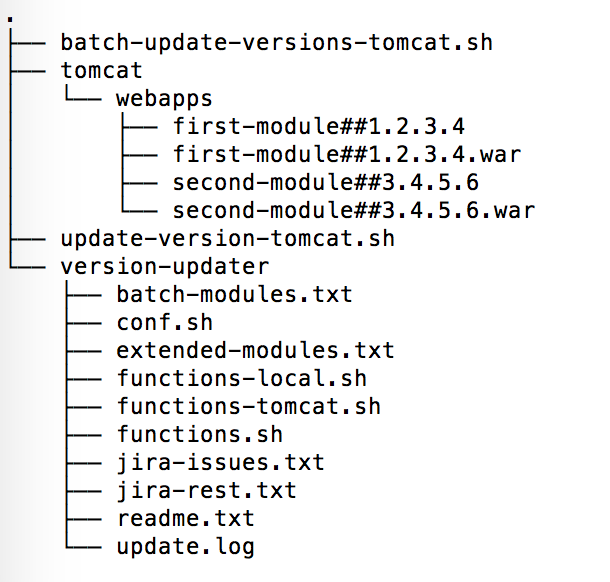
\includegraphics{screenshots/file-structure-on-tomcat.png}
      \caption*{\textit{Ekraanitõmmis 1: Skripti failide struktuur veebiserveriga Tomcat 8.}}
      \end{center}
   \end{figure}
   
   Failides \code{update-version-tomcat.sh}, \code{batch-update-versions-tomcat.sh}, \code{update-version-wl.sh} ja \code{batch-update-versions-wl.sh} on kirjeldatud skripti tööpõhimõte ehk mis tingimustel ja mis järjekorras on vaja käivitada funktsioone. Diagrammil 1 on näidatud protsessid, mis toimuvad ühe mooduli uuendamisel Tomcat 8 veebiserveril (faili \code{update-version-tomcat.sh} käivitamisel).
   
   \begin{figure}[H]
     \begin{center}
       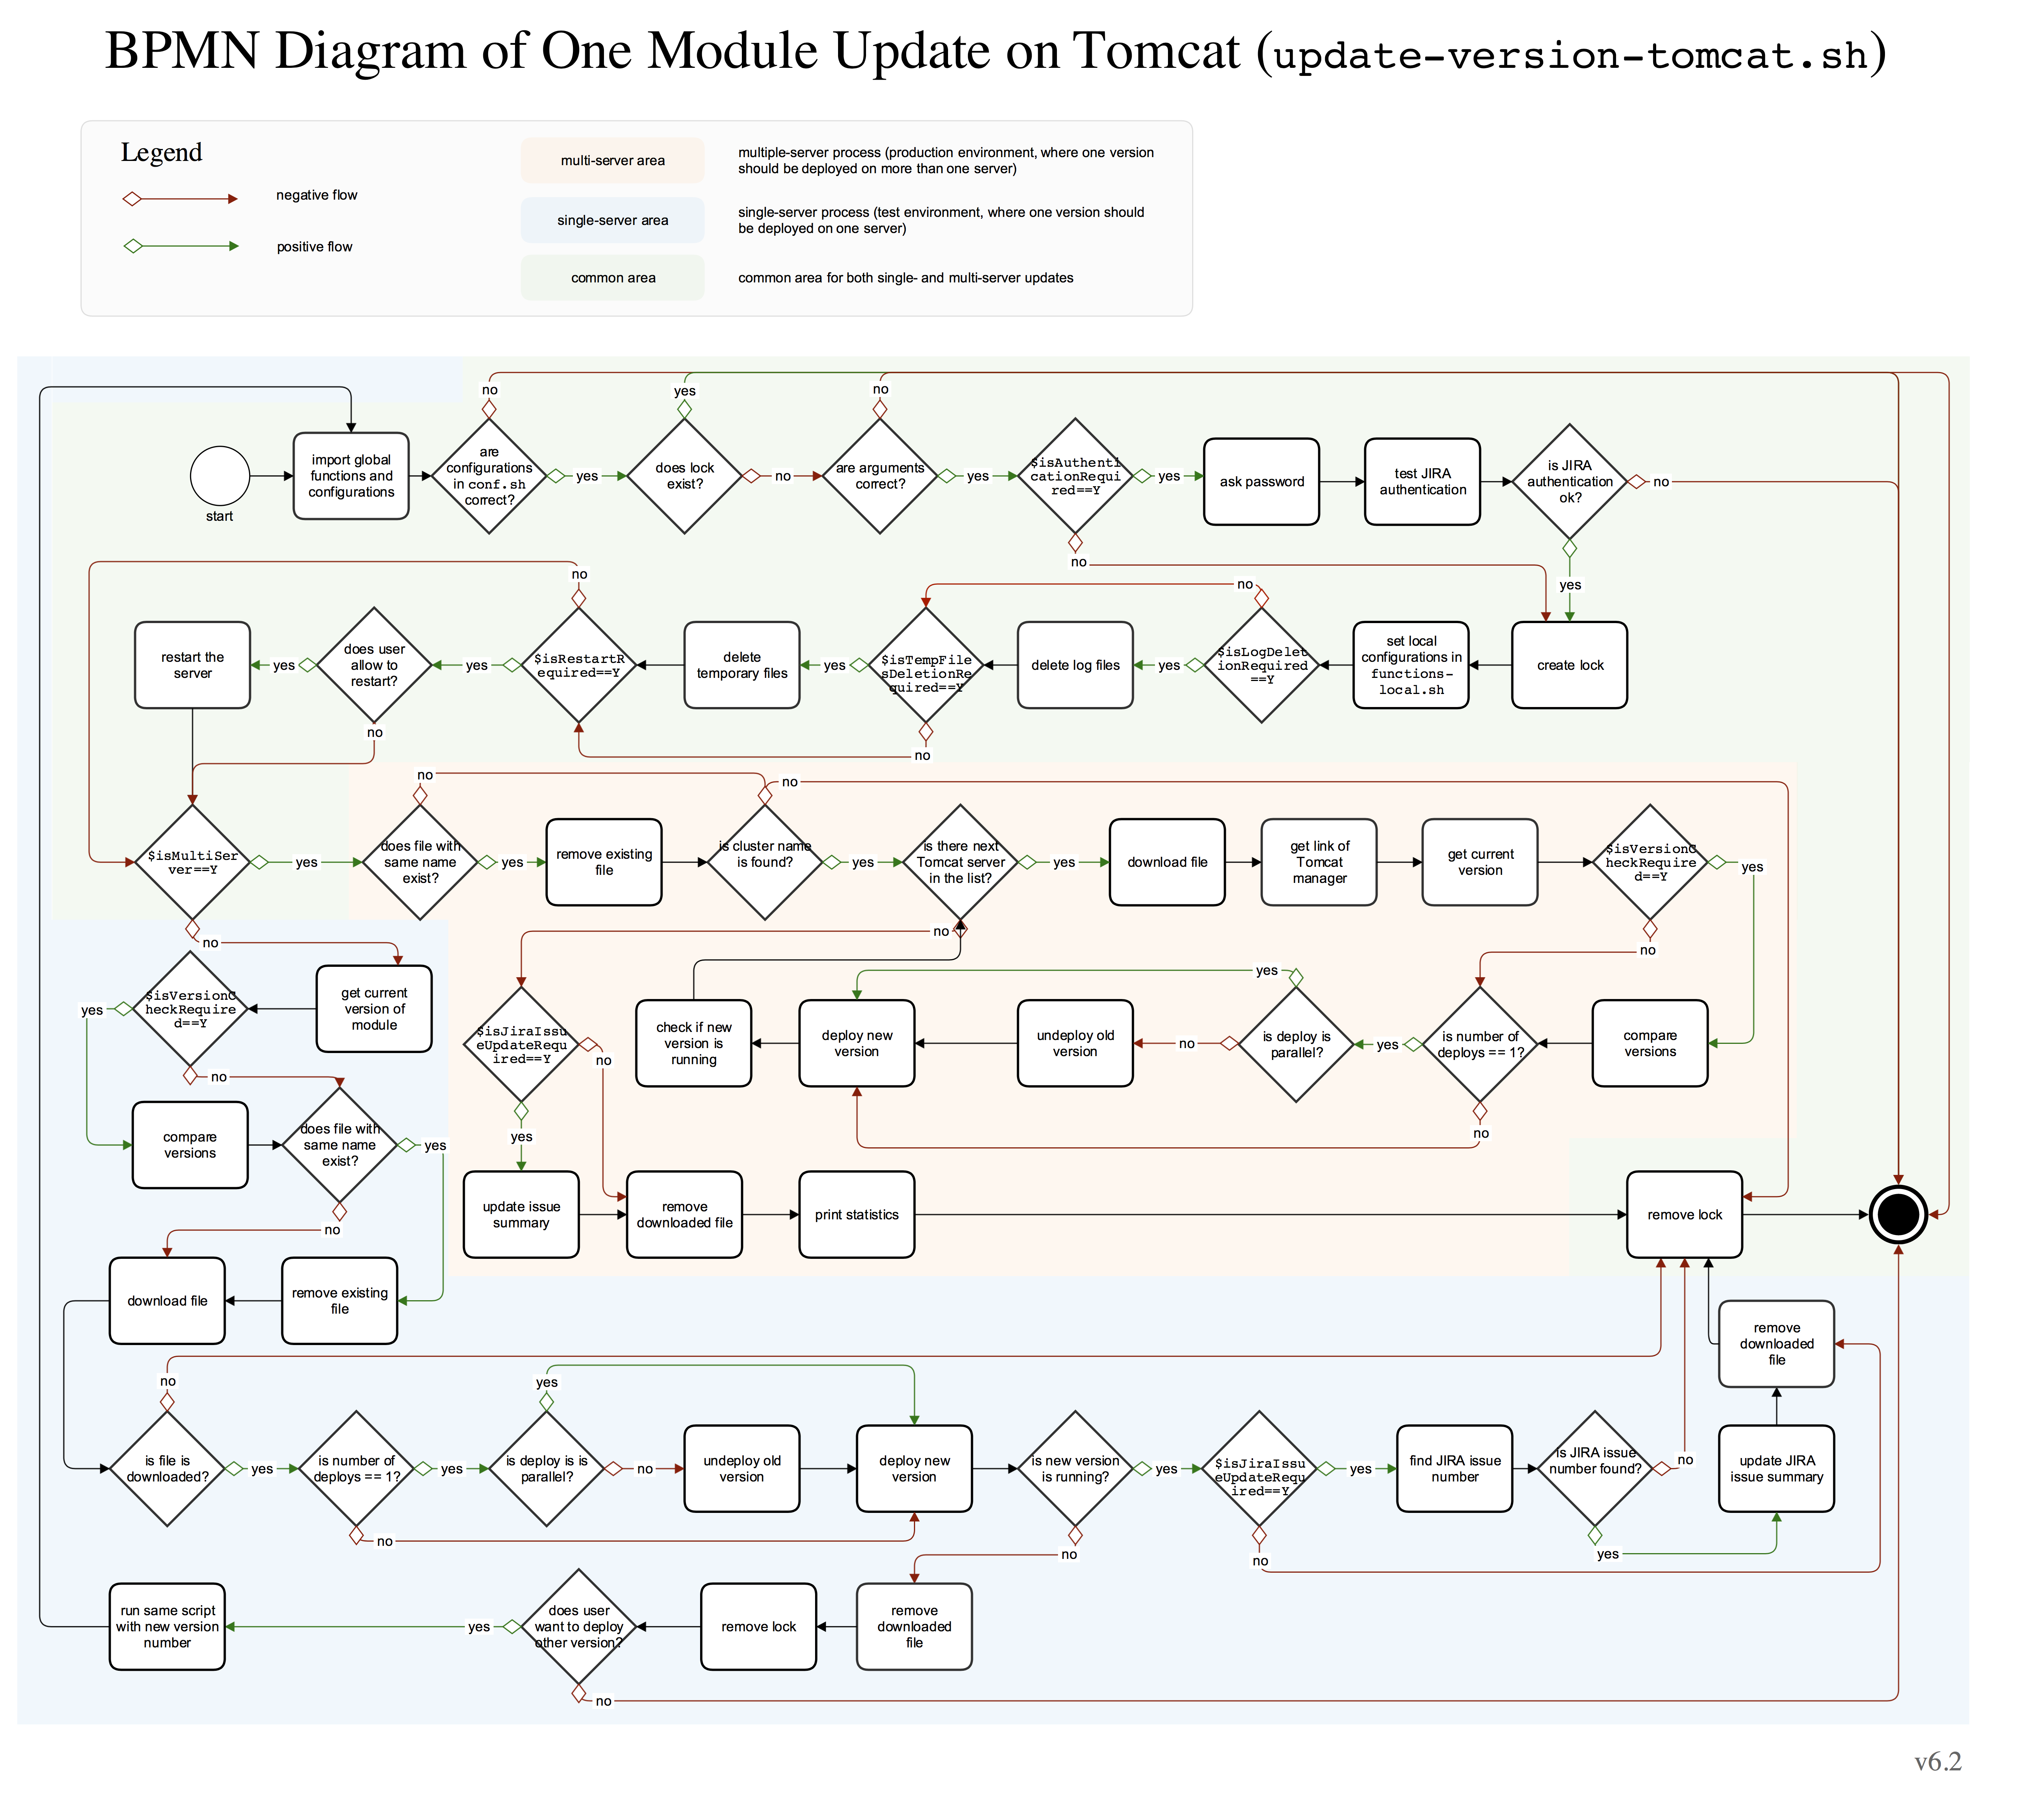
\includegraphics[width=\textwidth]{diagrams/BPMN-diagram-one-module-tomcat.png}
       \caption*{\textit{Diagramm 1: Skripti protsesside mudel ühe mooduli uuendamisel Tomcat 8 veebiserveril. Diagramm täissuuruses on kättesaadav järgmisel veebilingil: \url{https://iriiiina.gitbooks.io/version-updater-manual/content/BPMN-diagram-one-module-tomcat.png}}}
     \end{center}
   \end{figure}
   
   Diagrammil 2 on näidatud protsessid, mis toimuvad mitmete moodulite uuendamisel Tomcat 8 veebiserveril.
   
   \begin{figure}[H]
     \begin{center}
       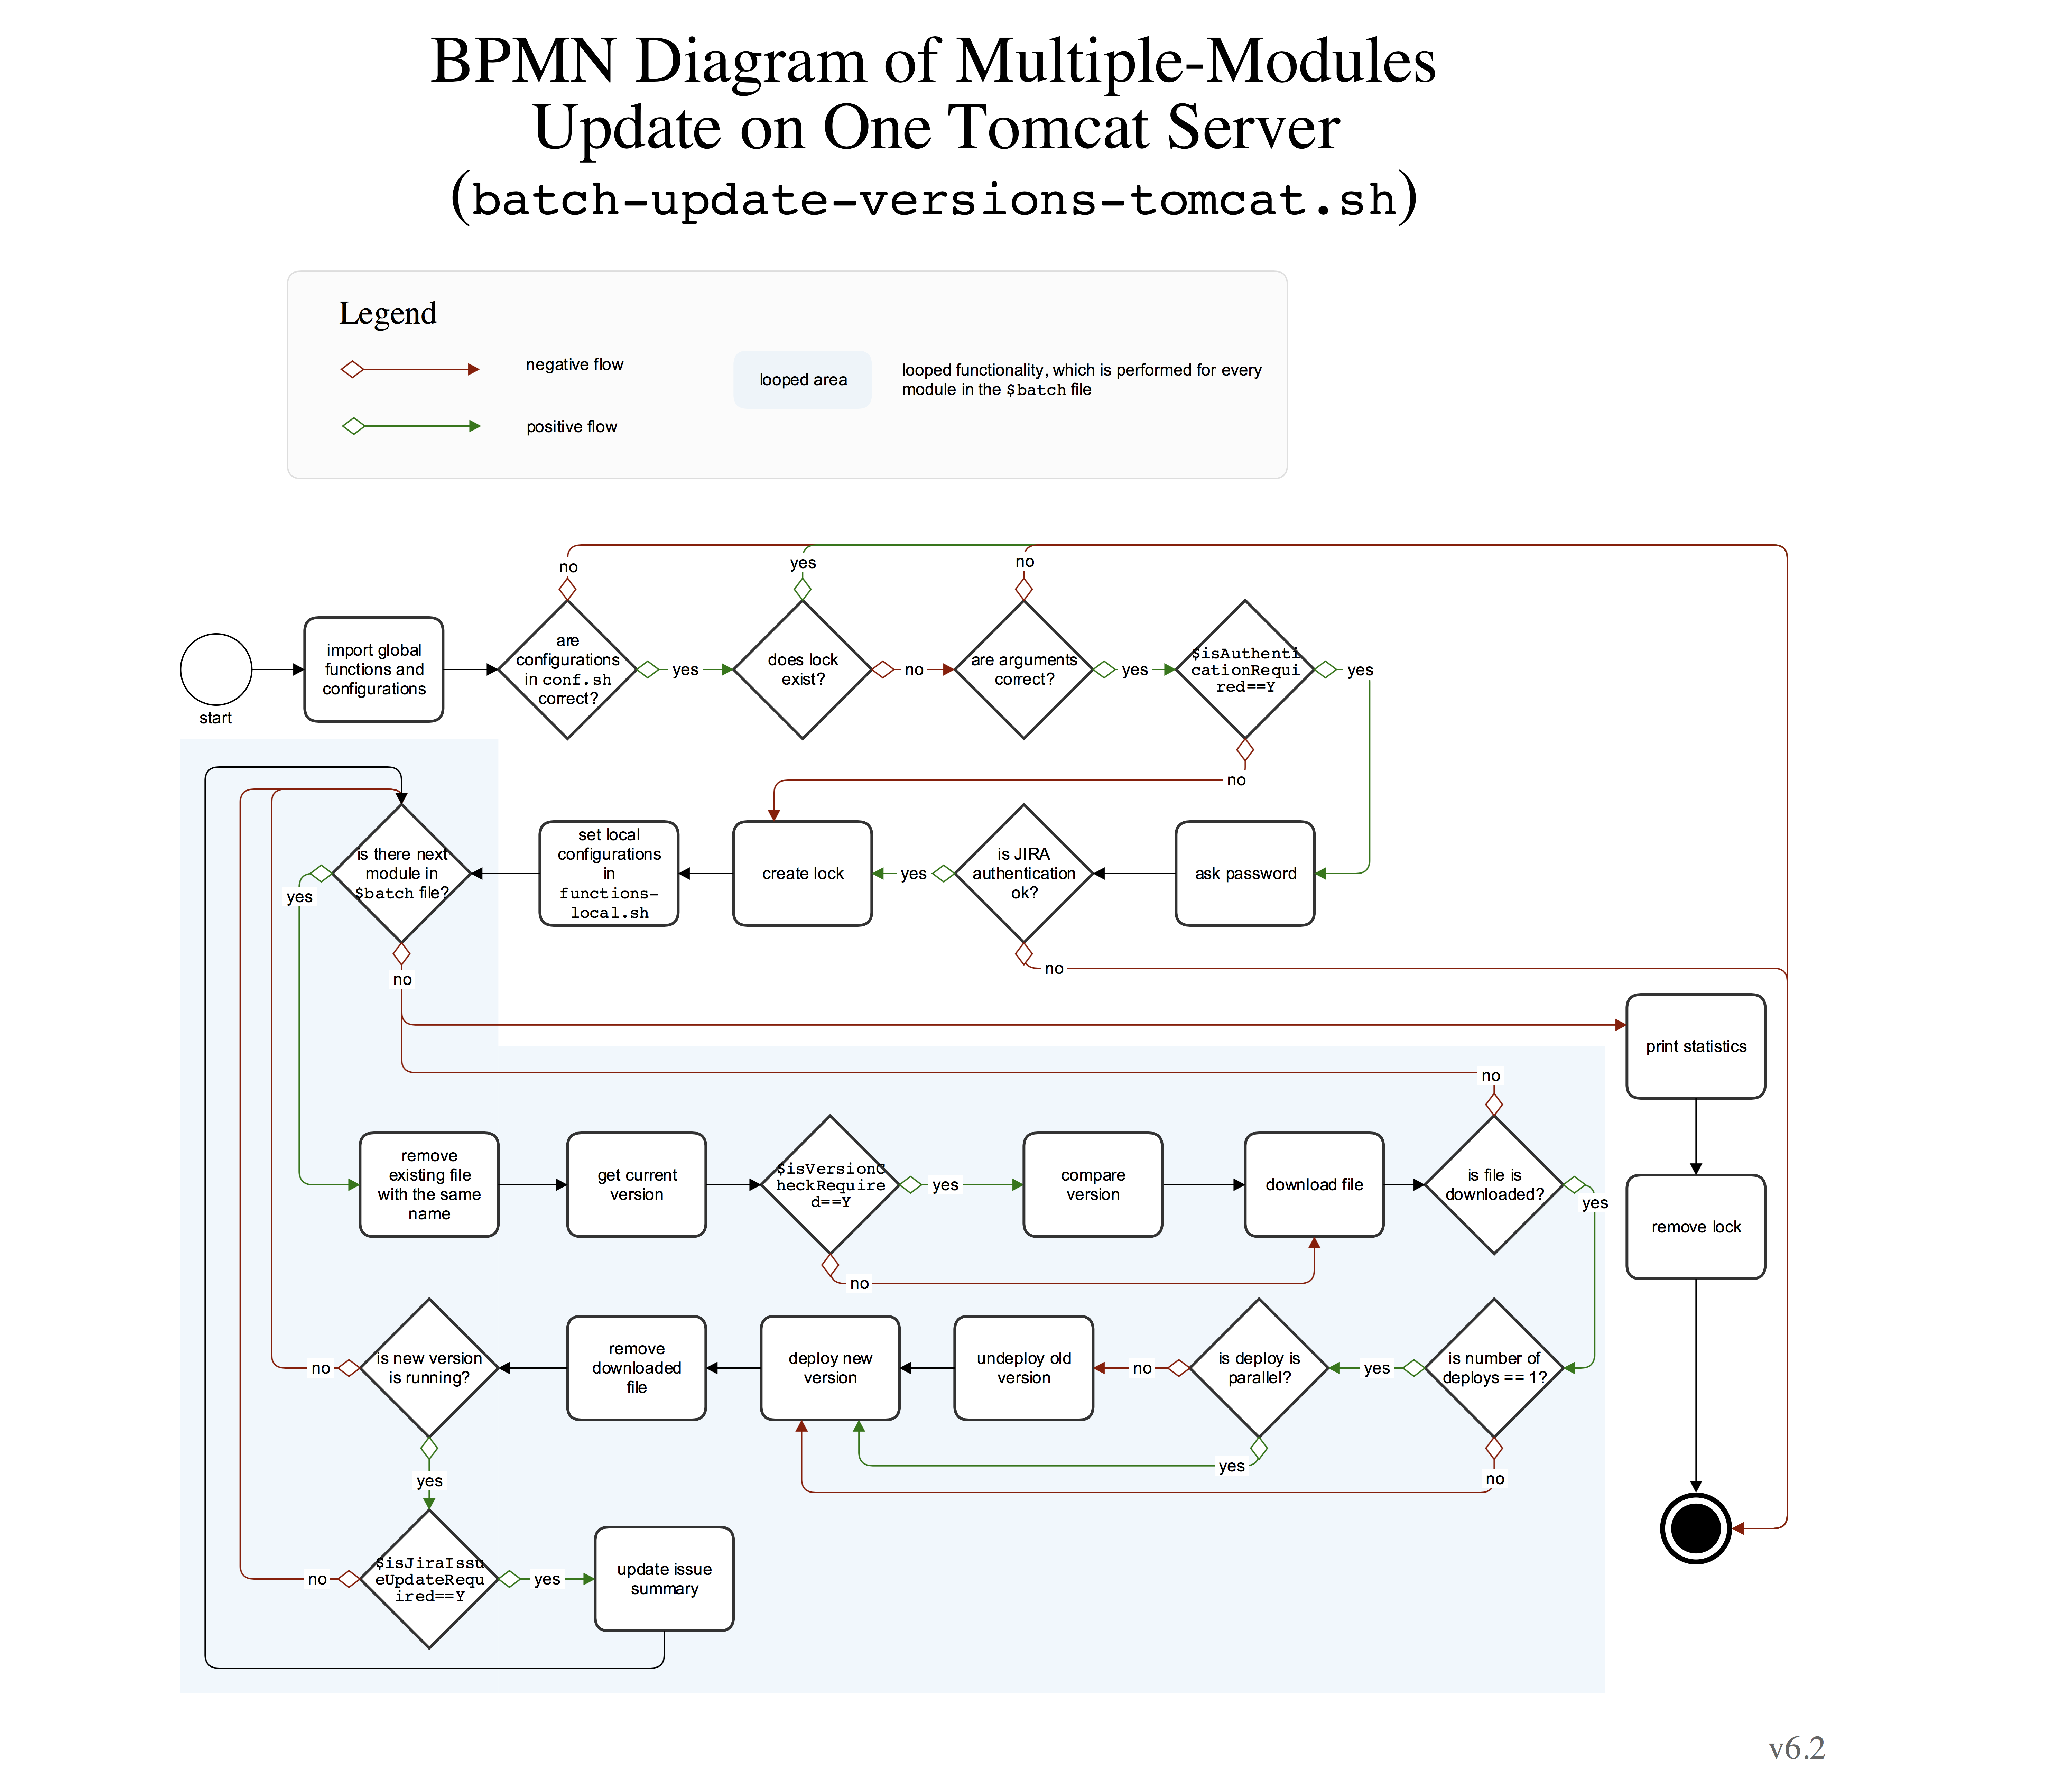
\includegraphics[width=\textwidth]{diagrams/BPMN-diagram-multiple-module-update-tomcat.png}
       \caption*{\textit{Diagramm 2: Skripti protsesside mudel mitmete moodulite uuendamisel Tomcat 8 veebiserveril. Diagramm täissuuruses on kättesaadav järgmisel veebilingil: \url{https://iriiiina.gitbooks.io/version-updater-manual/content/BPMN-diagram-multiple-module-update-tomcat.png}}}
     \end{center}
   \end{figure}

  Skriptil on olemas mõni funktsionaalsus, mis teeb selle kasutamist mugavamaks:
  
  \begin{itemize}
    \item Lukustamine \--- töö alguses skript kontrollib, kas serveril eksisteerib lukufail, kui mitte, siis tekitab seda ja jätkab tööd. Lukustamise loogika võimaldab vältida paralleelset uuendust sama veebserveri peal (lukufaili nimetust defineeritakse globaalse muutuja \code{\$lock} abil).
    
    \item Logimine \--- skript salvestab logid enda tegevuste kohta (globaalne muutuja \--- \code{\$log}).
    
    \item Skripti väljund on värviline, mis võimaldab lugeda seda kiiresti ja kohe märkada vigu.
    
    \item Skript teavitab kasutajat (kasutades terminali \code{\$bell} vahendit) juhtudel, kui see ootab mingit sisendit kasutaja poolt (näiteks, JIRA parooli) või kui skript lõpetas töö (mis võimaldab kasutajal mitte oodata tulemust).
    
    \item Mitmete moodulite uuendamisel või uuendamisel mitmete serverite peab sktipti töö lõpus näidatakse statistikat kõikide uuenduste seisust. See annab võimalust kohe aru saada uuenduse staatust ilma terve väljundi lugemata. Ekraanitõmmisel 2 on toodud kolme mooduli \code{system}, \code{authentication} ja \code{admin} uuenduse statistika, mis näitab, et kaks moodulit on uuendatud edukalt ja \code{system} mooduliga oli kaks probleemi: uue versiooni number \code{0.0.0.0} on väiksem, kus vana versiooni number \code{3.12.1.70} ja skriptil ei õnnestunud alla laadida uue versiooni faili \code{system-0.0.0.0}.
    \begin{figure}[H]
     \begin{center}
       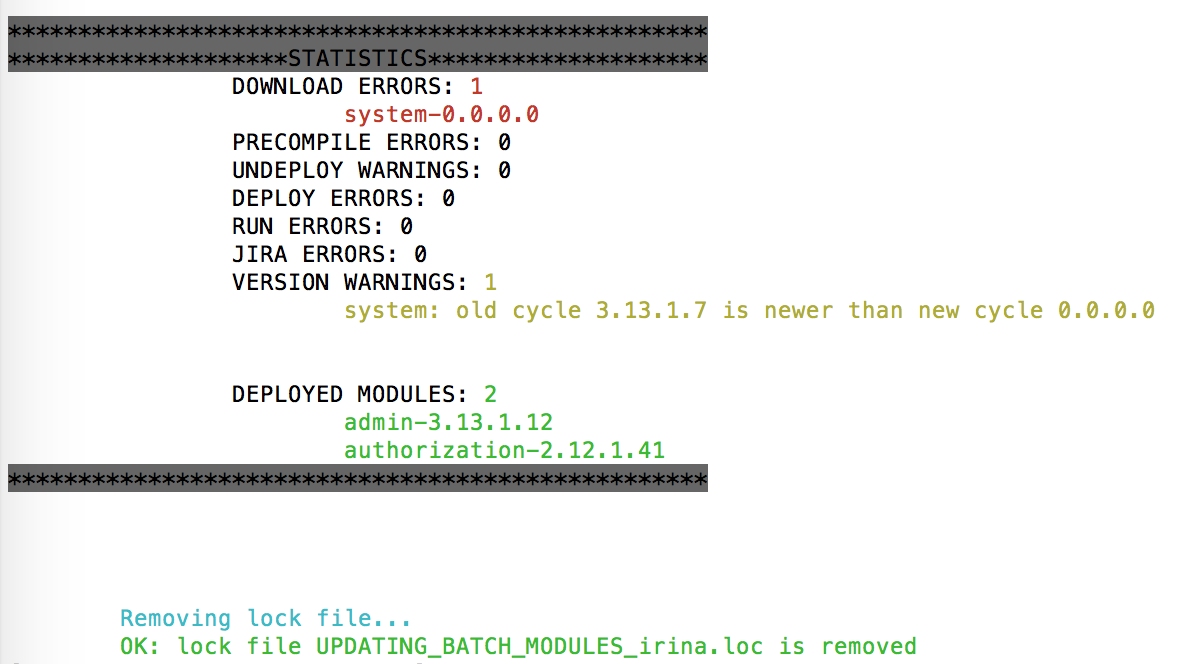
\includegraphics[width=.75\textwidth]{screenshots/statistics.png}
       \caption*{\textit{Ekraanitõmmis 2: Kolme mooduli uuenduse statistika.}}
     \end{center}
   \end{figure}
   
   \item Ühiseid faile on võimalik sünkroniseerida selleks, et nende parandus ja täiendus toimuks ainult ühes kohas. Selleks neid on vaja üles laadida reposetooriumisse ja seadistada serveril crontab \cite{cron} tööd, mis regulaarselt kontrolliks, kas reposetoorimuis on olemas faili uus versioon, kui on olemas, siis laadiks selle alla. Ekraanitõmmisel 3 on toodud näide crontab tööde kirjeldamisest.
   \begin{figure}[H]
     \begin{center} 
       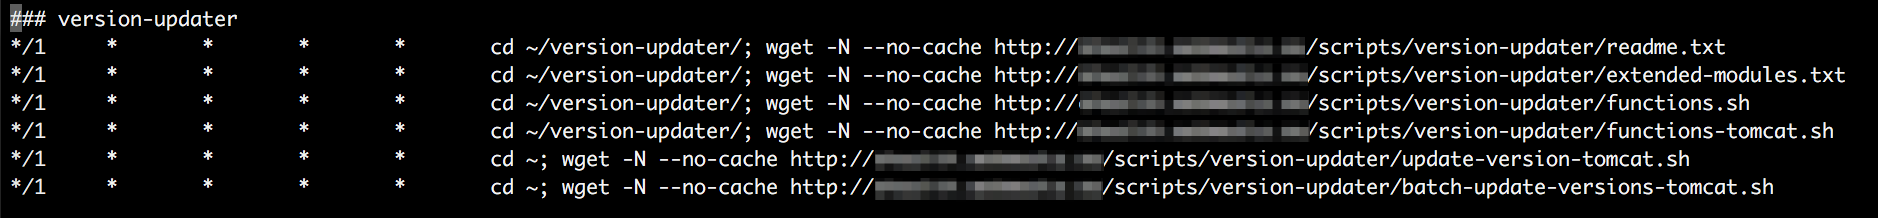
\includegraphics[width=.75\textwidth]{screenshots/crontab.png}
       \caption*{\textit{Ekraanitõmmis 3: Crontab tööde kirjelduse näide ühisfailide automaatse alla laadimiseks reposetooriumist.}}
     \end{center}
   \end{figure}
 \end{itemize}

  \subsection{Skripti paigaldus}
  
  Projekti reposetooriumis (ja avalikus GitHub reposetooriumis) on olemas kõik skripti failid, mida vajadusel saab alla laadida serveri, kohaliku või virtuaalmasina peale. Samuti on olemas \code{.zip} fail, kus on arhiveeritud kõik failid vastavalt skripti versioonile ja veebiserverile (on olemas eraldi arhiivid Tomcat ja WebLogic jaoks). Skripti paigaldamise protsess on kirjeldatud juhendis ja koosneb neljast sammust:
  \begin{itemize}
    \item Vastavata \code{.zip} faili alla laadimine serveri, kohaliku või virutaalmasina peale.
    \item Alla laaditud faili lahti pakkimine.
    \item Järgmiste failide täitmine serveri-spetsiifiliste andmetega:
    \begin{itemize}
      \item \code{version-updater/conf.sh}
      \item \code{version-updater/functions-local.sh}
      \item \code{version-updater/jira-issues.txt}
    \end{itemize}
    \item Crontab tööde seadistamine ühisfailide sünkroniseerimiseks.
  \end{itemize}
  
  \subsection{Skripti kasutus}
  
  Skripti käivitamiseks kasutatakse kaks faili: ühe mooduli uuendamiseks \code{update-version-*.sh} ja mitmete moodulite uuendamiseks \code{batch-update-versions-*.sh} (\code{*} asemel on \code{tomcat} või \code{wl}). Kõik ülejäänud failid skript kasutab enda töös ja kasutaja ei pea neid käivitama.\\
  
  Ühe mooduli uuendamise skriptile on võimalik anda 4 sisendparameetrit:
  \begin{center}
    \small{\code{./update-version-*.sh MODULE\_NAME MODULE\_VERSION JIRA\_USERNAME [p]}}
  \end{center}
  
  Näide:
  \begin{center}
    \small{\code{./update-version-tomcat.sh admin 1.1.1.1 irina}}
  \end{center}

  \begin{itemize}
    \item \code{MODULE\_NAME} \--- kohustuslik parameeter, mis määrab mooduli nimetust, mida soovitakse uuendada (näiteks, Tomcat-i puhul see on sama nimetus, mis \textit{path} Tomcat Manager-is).
    \item \code{MODULE\_VERSION} \--- kohustuslik parameeter, mis määrab versiooni, mida soovitakse paigaldada.
    \item \code{JIRA\_USERNAME} \--- parameeter on kohustuslik juhul, kui JIRA autentimine on kohustuslik (globaalne muutuja \code{\$isAuthenticationRequired="Y"}).
    \item \code{p} \--- mitte kohustuslik parameeter, mille sisestamisel teostatakse paralleelset uuendust (ei toimu vana versiooni eemaldamist).
  \end{itemize}\\
  
  Ekraanitõmmisel 4 on näidatud ühe mooduli edukas uuendus. Skript annab põhjaliku väljundi kõikidest sammudest, mis oli tehtud.
  
  \begin{figure}[H]
     \begin{center} 
       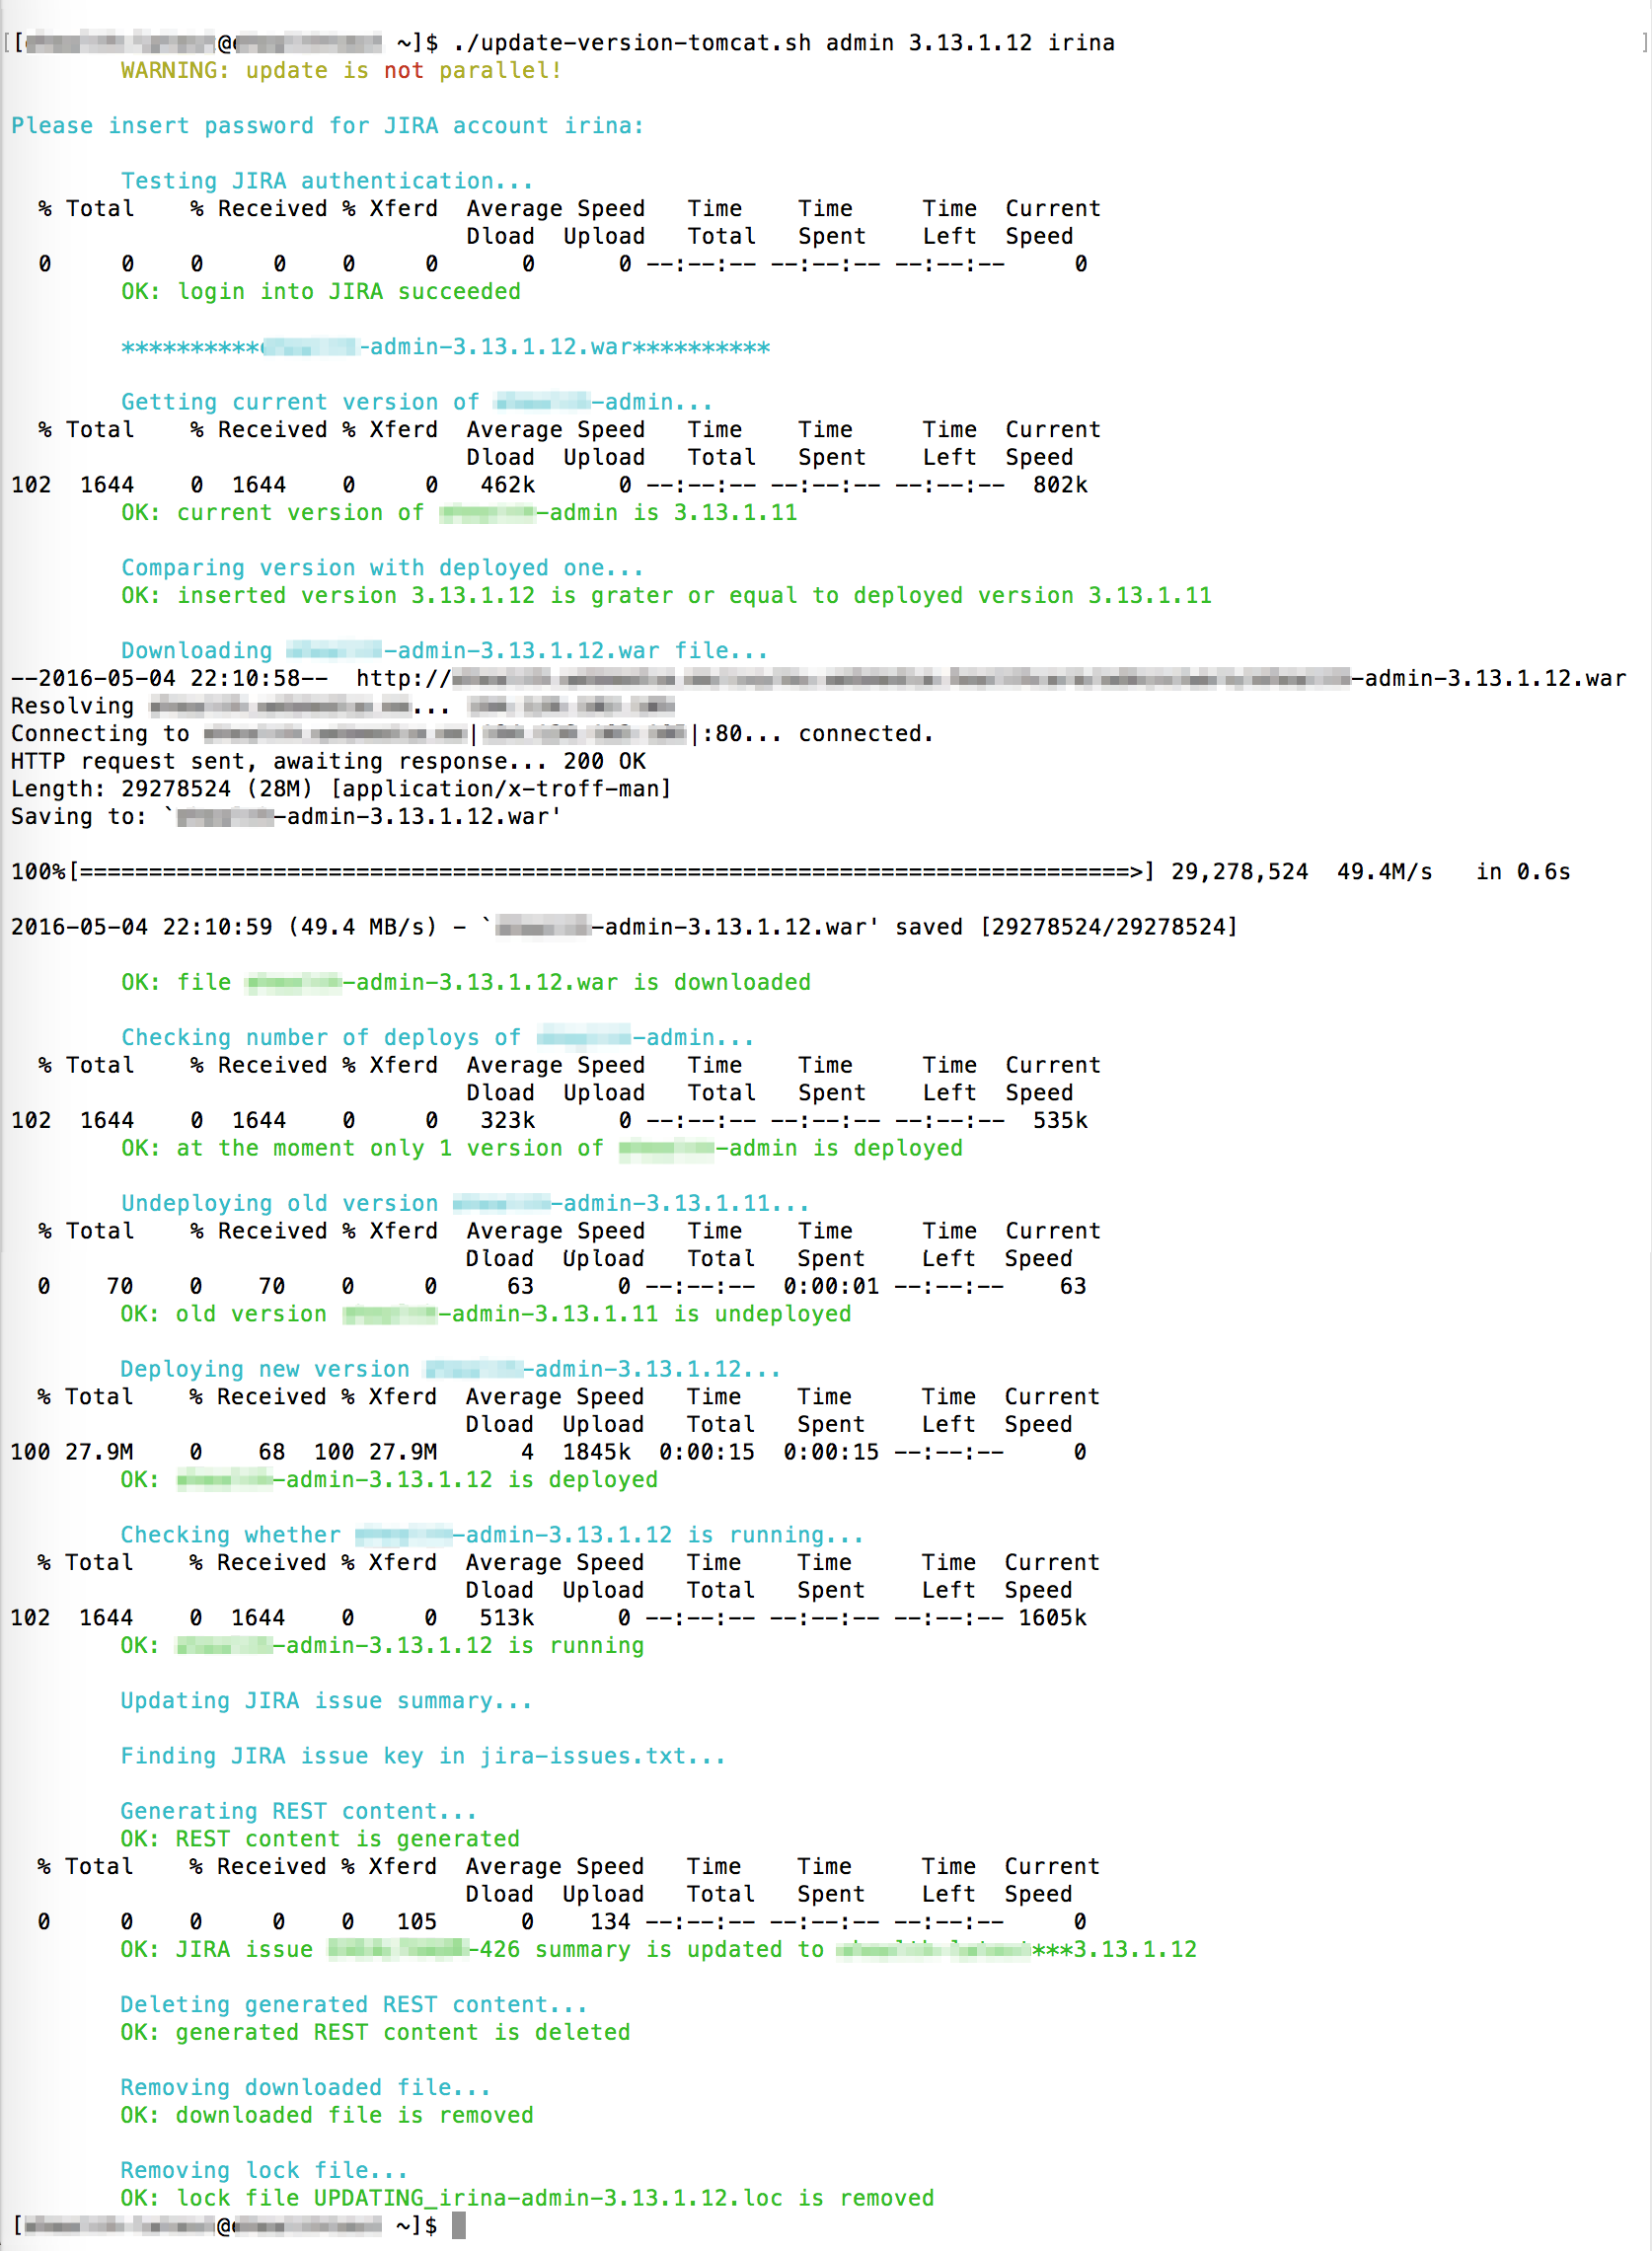
\includegraphics[width=\textwidth]{screenshots/one-module-successful-update.png}
       \caption*{\textit{Ekraanitõmmis 4: Ühe mooduli edukas uuendus skripti abil.}}
     \end{center}
   \end{figure}
  
  Mitmete moodulite uuendamise skriptile on võimalik anda 2 sisendparameetrit:
  
  \begin{center}
    \small{\code{./batch-update-versions-*.sh JIRA\_USERNAME [p]}}
  \end{center}
  
  Näide:
  \begin{center}
    \small{\code{./batch-update-versions-tomcat.sh irina p}}
  \end{center}
  
  \begin{itemize}
    \item \code{JIRA\_USERNAME} \--- parameeter on kohustuslik juhul, kui JIRA autentimine on kohustuslik (globaalne muutuja \code{\$isAuthenticationRequired="Y"}).
    \item \code{p} \--- mitte kohustuslik parameeter, mille sisestamisel teostatakse paralleelset uuendust (ei toimu vana versiooni eemaldamist).
  \end{itemize}

  \subsection{Dokumentatsioon}
  
  Skripti kohta on olemas põhjalik dokumentatsioon, mis on uuenduse raamistiku oluline osa. Skripti juhend kirjeldab seda, kuidas saab kasutada, paigaldada ja seadistada skripti. Juhend on kätte saadav kõikidele meeskonna liikmetele, mis tähendab, et iga ühel on olemas võimalus seda kasutada. Mõlemad skripti projekti juhend ja avalik juhend on kättesaadavad töö lisas.
  
  \newpage
  
  % Mõju projektile
  \section{Mõju projektile}
  
  Automaatne versiooni uuenduse raamistik täielikult asendas vana käsitsi protsessi. Selles on olemas nii eelised, kuid ka oma puudused.\\
  
  Kõige oluline eelis on see, et skript täidab kõik nõuded tabelist 2 "Nõuded versiooni uuenduse lihtsustamise lahendusele". Kõige märkavamad nendest on nõuded 1 ja 2 \--- protsessi kiirus ja mugavus.\\
  
  On mõõdetud vana ja uue uuenduse protsesside kiirused. Automaatse protsessi alguseks oli võetud skripti käivitamise käsku kirjutamine ja lõppuks skripti teavitamine, et töö on lõppenud. Skripti töö aja mõõtmiseks oli kasutatud \textit{UNIX} käsurea funktsioon \code{time} \cite{time}. Käsitsi uuenduse protsess koosneb sammudest, mis on kirjeldatud tabelis 1 "Manuaalse uuenduse protsessi sammud" ja kulutud aeg oli mõõdetud stopperiga.\\
  
  Oli valitud 4 protsessi, mis olid teostatud samal serveril ja samade .WAR failidega: 3 üksikute kõige populaarsemate moodulite uuendamine ja kõikide moodulite uuendamine (võetud keskkonnas neid oli 18 tk). Iga protsess oli tehtud vana käsitsi viisi ja uue automaatse skriptiga 3 korda ja võrdluseks on võetud katsetuste keskmised väärtused. Tulemused on toodud tabelis 4 "Vana ja uue protsesside kiirused".
  
  \begin{table}[!htbp]
    \begin{center}
      \begin{tabular}{| l | c | c |}
        \hline
         \textbf{Moodul} & \textbf{Aut. uuendus} & \textbf{Käsitsi uuendus}\\
        \hline
        admin & 27s & 80s\\
        treatment & 61s & 112s\\
        reception & 38s & 100s\\
        kõik (18 tk) & 9m 12s & 34m 8s\\
        \hline
      \end{tabular}
      \caption*{\textit{Tabel 4: Vana ja uue protsesside kiirused}}
    \end{center}
  \end{table}
  
  Tegelikkuses kokkuhoidud aeg on veel suurem, sest vanas protsessis uuendaja tähelepanu oli hõivatud terve protsessi jooksul. Uue skripti kasutades testijatel on olemas võimalus tegeleda paralleelselt teiste ülesannetega ja mitte jälgida skripti tööd (see ise annab teada, kui uuendus on lõppenud).\\
  
  Kõige oluline puudus on see, et testijad enam ei tunne versiooni uuenduse protsessi tausta ja vigade tekitamise juhul (kas serveri, veebiserveri või skripti pärast) ei oska neid lahendada. See on üldine automatiseerimise probleem, millega tuleb lepida mugavuse vahetuseks.\\
  
   Käesoleva töö raames oli küsitud tagasiside uue raamistiku kohta meeskonnaliikmete käest, kes on seda kasutanud. Allpool on toodud mõned väljavõted, terved tekstid on kättesaadavad lisas 5.5.\\
   
   \begin{displayquote}
   ``I also like that scalability has been considered when writing the script + many optional features have been implemented which can be used if one desires to do so.'' (Martin Rakver, Hosting Services and Application Manager)
   \end{displayquote}
   
   \begin{displayquote}
   ``I personally think that version-update script has significantly improved the speed of version update.'' (Kalle Jagula, QA Specialist)
   \end{displayquote}
   
   \begin{displayquote}
    ``Version updater script has standardized the way our environments are updated, reducing learning curve for new people performing the task. Downside is that people are unaware, what happens in the background and can't handle simple errors in the process anymore.'' (Tanel Käär, System Architect)
    \end{displayquote}
    
    \begin{displayquote}
    ``The scripts allowed me to conveniently perform the updates while letting me concentrate on solving the primary problems and not leaving the environment containing all necessary information.'' (Klaus-Eduard Runnel, Senior Programmer)
    \end{displayquote}
    
    \begin{displayquote}
    ``Samuti tooks välja, et uuendamise skriptid on väga hästi dokumenteeritud ja põhjalikult kirja pandud kuidas toimivad.'' (Helina Ziugand, QA Specialist)
    \end{displayquote}

  \newpage
  
  % Lahenduse perspektiivid
  \section{Lahenduse perspektiivid}
  
  Bash skripti kood Apache Tomcat veebiserveri jaoks on avalik ja asub \textit{GitHub} reposetooriumis \url{https://github.com/iriiiina/version-updater}. See tähendab, et igaüks, kellel on sarnane takrvaraarenduse süsteem, saab seda kasutada ja täiendada enda nõuete järgi. Iga faili sees on olemas põhjalikud kommentaarid, mis seletavad faili eesmärki ja selle kasutamisviisi, mis lihtsustab skripti arusaamist. Samuti \textit{GitHub} platvormil on olemas võimalus raporteerida vigu ja tellida uut funktsionaalsust.\\
  
  Nõuded Bash skripti avaliku versiooni kasutamiseks:
  \begin{itemize}
    \item Masin, kus on paigaldatud Bash vahend.
    \item Apache Tomcat 8 veebiserver (vajadusel skripti saab muuta Tomcat 7 ja 6 versioonide jaoks).
    \item Standartsed \textit{UNIX} vahendid: \code{find}, \code{grep}, \code{wget} (kui mooduli failid asuvad veebis), \code{curl}.
    \item Standartne käsurea \code{bell} funktsionaalsus, mis saadab teavitusi kasutajale terminali kaudu.
  \end{itemize}\\
  
  Lisaks skriptil on olemas avalik dokumentatsioon, mis asub \textit{GitBook} reposetooriumis \url{https://iriiiina.gitbooks.io/version-updater-manual/content/}. See sisaldab kasutusjuhendit, paigaldamise ja seadistamise juhendit ja kirjeldab kuidas on võimalik laiendata skripti tööd standartsete \textit{UNIX} vahenditega.\\
  
  Koodi ja dokumentatsiooni avalikkus tähendavad mitte ainult seda, et igaüks saab rakendada seda omas projektis, aga ka olemas oleva lahenduse optimiseerimist ja uue funktsionaalsusega täiendamist.
  
  \newpage
  
  % Kokkuvõte
  \section*{Kokkuvõte}
  \label{kokkuvote}
  \addcontentsline{toc}{section}{\nameref{kokkuvote}}
  
  Käesoleva bakalaureusetöö eesmärgiks oli automatiseerida versiooniuuenduse protsessi konkreetses projektis, selleks, et lihtsustada antud protsessi, et säästa aega ja vähendada inimlike vigade arvu.\\
  
  Bakalaureusetöö teoreetilise osa käigus koostati 12 nõuet probleemi lahendusele ja uuriti 4 erinevat tööriista versiooni uuenduse haldamiseks. Mitte ükski neist ei vastanud kõikidele nõuetele. Lahenduseks valiti enda Bash skripti kirjutamist.\\
  
  Bakalaureusetöö praktilise osa käigus oli kirjutatud Bash skript versioonide uuendamiseks, mis vastab kõikidele nõuetele. Oli tehtud ka põhjalik juhend selle skripti paigaldamise, seadistamise ja kasutamise kohta.\\
  
  Bakalaureusetöö püstitatud eesmärgid said täidetud ning kirjutatud Bash skript aitab kiiremini ja mugavam uuendada versioone projektis. Seda kinnitavad meeskonnaliikmete tagasiside ja vana ja uue protsesside aegade võrdlemine.\\
  
  Loodud lahendust saavad kasutada ja täiendada ka teised projektid, kuna selle kood ja dokumentatsioon on avalikud.

  \newpage
  
  % Kasutatud materjalid 
  \begin{thebibliography}{9}
    \label{kasutatud-materjalid}
    \addcontentsline{toc}{section}{\nameref{kasutatud-materjalid}}
  
    \bibitem{bash}
    \url{https://www.gnu.org/software/bash/manual/bashref.html}
    
    \bibitem{tomcat}
    \url{https://tomcat.apache.org/tomcat-8.0-doc/manager-howto.html}
  
    \bibitem{cron}
    \url{https://help.ubuntu.com/community/CronHowto}
  
    \bibitem{hg}
    \url{https://www.mercurial-scm.org/guide}
  
    \bibitem{centos}
    \url{https://wiki.centos.org/FrontPage}
  
    \bibitem{bamboo}
    \url{https://www.atlassian.com/software/bamboo}
  
    \bibitem{chef}
    \url{https://www.chef.io}
  
    \bibitem{jenkins}
    \url{https://jenkins-ci.org}
  
    \bibitem{ansible}
    \url{https://www.ansible.com}
    
    \bibitem{time}
    \url{http://pubs.opengroup.org/onlinepubs/9699919799/utilities/time.html}
 
  \end{thebibliography}

  \newpage
  
  % Lisad
  \section*{Lisad}
  \label{lisad}
  \addcontentsline{toc}{section}{\nameref{lisad}}
  
  \subsection*{Terminid}
  
  \textbf{Raamistik (\textit{framework})} \--- süsteem, mis kirjeldab protsessi teostamist. Töö raames raamistiku all mõeldatakse Bash skripti koodi ja selle dokumentatsiooni.\\
  
  \textbf{Server} \--- riistvara- ja tarkvarasüsteem, kus on paigaldatud veebiserver.\\
  
  \textbf{Veebiserver} \--- klient-server-mudelil ja protokollil HTTP või HTTPS põhinev tarkvara, mis võtab vastu kasutajate brauseritelt tulevaid päringuid ja saadab vastuseks HTML-lehti ja faile (nt Apache Tomcat või Oracle WebLogic) (http://akit.cyber.ee/term/3152-veebiserver).\\
  
  \textbf{Rakendus (\textit{application})} \--- tarkvara, mis on paigaldatud veebiserveril ja on kättesaadav kasutamiseks.\\
  
  \textbf{Test rakendus} \--- rakendus, mida projekti meeskonnaliikmed kasutavad tarkvara testimiseks.\\
  
  \textbf{Demo rakendus} \--- rakendus, mida kliendid kasutavad funktsionaalsuse testimiseks.\\
  
  \textbf{Toodang rakendus} \--- lõppkasutajate rakendus.\\
  
  \textbf{Moodul} \--- tarkvara osa, kus on kogutud ja pakitud ühe funktsionaalsuse kood (üks .WAR fail on üks moodul)\\
  
  \textbf{Versioon} \--- number, mis määrab .WAR faili sisu (.WAR fail sisaldab funktsionaalsust ja parandusi vastavalt versiooni numbrile).\\
  
  \textbf{Modulaarne süsteem} \--- tarkvaraarenduse süsteem, mille korral kogu koodi jagatakse moodulite kaupa, selleks, et ühe funktsionaalsuse tarnimine ei nõuaks terve rakenduse uuendamist.\\
  
  \subsection*{Skripti lähtekood}
  
  Bash skripti kood asub avalikus GitHub reposetooriumis:\\
  \url{https://github.com/iriiiina/version-updater}
  
  \subsection*{Skripti avalik juhend}
  
  Bash skripti avalik juhend asub avalikus GitBook reposetoorimus:\\
  \url{https://iriiiina.gitbooks.io/version-updater-manual/content/}
  
  \subsection*{Skripti projekti juhend}
  
  Bash skripti projekti sisene juhend:\\
  \url{https://github.com/iriiiina/bachelors-thesis/blob/master/manual/Confluence%20Manual.pdf}
  
  \subsection*{Kolleegide tagasiside}
  
  \subsubsection{Martin Rakver, Hosting Services and Application Manager}
  
  I have not been using the script very much, because I rarely update modules nowadays. But what I can say is that it is definately in the right place – automating activities that testers would need do to on daily basis each time when deploying a new module. Come to think about it, there are actually quite many activites related to new module deployment – would be interesting to compare the time it takes to deploy a module manually vs using script + calculate about how much time we as a team are saving daily, montly, yearly (and get to do more important things with that time).
I also like that scalability has been considered when writing the script + many optional features have been implemented which can be used if one desires to do so.

  \subsubsection{Kalle Jagula, QA Specialist}
  
  I personally think that version-update script has significantly improved the speed of version update. Especially with the settings for bulk-update, which improves the speed of modules' version update and manageability of test/demo environments.
  
  \subsubsection{Tanel Käär, System Architect}
  
  Version updater script has standardized the way our environments are updated, reducing learning curve for new people performing the task. Downside is that people are unaware, what happens in the background and can't handle simple errors in the process anymore.
  
  \subsubsection{Klaus-Eduard Runnel, Senior Programmer}
  
  I have mostly used the scripts to perform quick module and dependency updates in specific test environments when deploying quick fixes or debugging problems in the modules I'm responsible for. Deployment of artifacts is secondary task in such scenarios. The scripts allowed me to conveniently perform the updates while letting me concentrate on solving the primary problems and not leaving the environment containing all necessary information.

In some cases it was necessary to deploy custom-built experimental (unversioned) war-files. In these cases the scripts could not be used.
They would have been useful though if such experiments would have been commited to feature branches and published as feature branch artifacts. (As of today, we are better prepared for such circumstances.)

The scripts were also useful to deploy predefined sets of modules to temporary test environments living on reusable virtual machine images. It is important to note that a module update triggers launching a set of associated sql scripts to bring a database schema up to date. In that way the version update scripts let us automate most of a process of setting up updated environment from virtual machine images.

It would be helpful if the scripts were adapted to perform changes on remote machines and to perform changes on multiple environments simultaneously.

  \subsubsection{Helina Ziugand, QA Specialist}
  
  Uuendamise skriptid on nii projektile kui ka minu igapäevasele tööle väga positiivselt mõjunud. 
Kui algselt oli uuendamise jaoks vaja mitu sammu käsitsi teha, siis nüüd käib see automaatselt ja kiiresti. Võiks öelda, et üsna tüütu oli alguses kogu see uuendamise protsess - pidevalt pidi jälgima, kas vaja käsureale kirjutada järgmist sammu, hiljem JIRAs vana versiooni numbrit muuta ja Weblogicust vana versioon kustutada. Praegu on väga mugav ühe käsklusega uuendamise skript tööle panna, mis korraga kõik vajalikud sammud ära teeb ja samal ajal kui skript jookseb ise teiste tegevustega jätkata. Väga selgelt erinevate värvidega on välja tootud error, warningu ja success teated, mis on lihtsasti märgatavad ja hästi loetavad. 

Kui vaja on rohkem kui ühte moodulit uuendada, siis väga hea lahendus on selleks mitme moodulise uuendamise skript. Kui varem oli vaja keskkonda uue tsükli peale uuendada, siis võttis see ebamugavalt kaua aega ja vabatahtlikult kõige parema meelega seda ette ei tahtnud võtta. Nüüd on vaja ainult uuendatavad versioonid tekstifaili kirja panna ja ühe käsklusega skript käima tõmmata. 

Samuti tooks välja, et uuendamise skriptid on väga hästi dokumenteeritud ja põhjalikult kirja pandud kuidas toimivad. Mul on väga hea meel, et versioonide uuendamine on skriptide abil nii lihtsaks, mugavaks ja meeldivaks tegevuseks saanud.

  \newpage

  \subsection*{Litsents}
  
  \textbf{Lihtlitsents lõputöö reprodutseerimiseks ja lõputöö üldsusele kättesaadavaks tegemiseks}\\
  
  Mina \textbf{Irina Ivanova} (sünnikuupäev: 9.05.1988)
  \begin{enumerate}
    \item annan Tartu Üikoolile tasuta loa (lihtlitsentsi) enda loodud teose \textbf{Versiooniuuenduse raamistik kasutades skriptimiskeelt Bash}, mille juhendajad on Helle Hein ja Polina Morozova,
    \begin{enumerate}
      \item reprodutseerimiseks säilitamise ja üldsusele kättesaadavaks tegemise eesmärgil, sealhulgas digitaalarhiivi DSpace-is lisamise eesmärgil kuni autoriõiguse kehtivuse tähtaja lõppemiseni;
      \item üldsusele kättesaadavaks tegemiseks Tartu Ülikooli veebikeskkonna kaudu, sealhulgas digitaalarhiivi DSpace-i kaudu kuni autoriõiguse kehtivuse tähtaja lõppemiseni.
    \end{enumerate}
    \item olen teadlik, et punktis 1 nimetatud õigused jäävad alles ka autorile.
    \item kinnitan, et lihtlitsentsi andmisega ei rikuta teiste isikute intellektuaalomandi ega isikuandmete kaitse seadusest tulenevaid õigusi.
  \end{enumerate}
  
  Tartus, 1.05.2016

\end{document}